\chapter{Background}\label{background}

Generally speaking, estimation of the function that outputs the neural response corresponding to an auditory stimulus has been heavily studied, given its theoretical and practical importance regarding the computational modeling of the brain. A fundamental goal of systems neuroscience is to understand and model the stimulus-response processing that takes place as electrical signals are transmitted through the brain. As opposed to emotion or the sense of self, the study of the perceptual system (visual/auditory/tactile etc.) has the distinct advantage that the input is easily observable and controllable, allowing for systematic exposure to very specific stimuli. 

Therefore, various stimuli and mathematical methods have been devised in order to optimally estimate the stimulus-response function of a neuron. \textcite{meyerModelsNeuronalStimulusResponse2017} gives an overview of these models, each with the corresponding statistical estimation methods. I will be explaining selected models below, in order to put the research into context and aid understanding of the evolution of these techniques.

\section{Models and estimation methods}

\subsection{Gaussian linear model}

The Gaussian linear model assumes that the response is a linear combination of the stimulus, therefore that:

\begin{equation*} \label{LM}
\hat{r}(t) = \mnot{k^{T}}\mnot{s}(t) + \epsilon(t) = \sum_{i=1}^D k_i s_i(t)  + \epsilon(t) = k_1 s_1(t) + k_2 s_2(t) + k_3 s_3(t) + \ldots + k_D s_D(t) +  \epsilon(t) 
\end{equation*}
where $\mnot{s}(t)$ represents the stimulus spectrogram, containing $D$ vectors of length $s_{length}$, one for each time unit, and $\mnot{k}$ contains $D \times s_{length}$ weights. Therefore, in the case of a spectrogram input, each instance in the discrete time $\times$ frequency bin space has a corresponding weight in the weight matrix (filter) $\mnot{k}$.

In the Gaussian linear model, normally distributed noise $\epsilon(t) \sim \mathcal{N}(0, \sum^2)$ is added to the estimated response above, in order to model response variability \parencite{meyerModelsNeuronalStimulusResponse2017}.

\subsection{Linear-Nonlinear (LN) cascades}

Compared to the Gaussian linear model, the cascade models transform the response $\mnot{k^T}\mnot{s}(t)$ using a memoryless function $f$:

\begin{equation}
	\hat{r} = f(\mnot{k^T}\mnot{s}(t))
\end{equation}

Function $f$ is memoryless, meaning that it acts exclusively in the moment $t$, without using information from the past or from the future.

\subsection{Spectrotemporal receptive fields (STRFs)}

\subsubsection{Mathematical representation}

As per \textcite{aertsenSpectroTemporalReceptiveField1981}, a stimulus-invariant system can be exemplified by the linear system, which takes an input $x(t)$ and computes the output $y(t)$:

\begin{equation*}
	y(t) = \int \mathrm{d}\tau h(\tau) x(t - \tau)
\end{equation*}

The operation illustrated above is called \emph{convolution}, and the function $h(t)$ which relates the input $x(t)$ to the output $y(t)$ is the \emph{impulse response}. The system is called stimulus-invariant because the same transformation is applied all stimuli, independently of their characteristics.

As described in \textcite{aertsenSpectrotemporalReceptiveFields1980}, the spectrotemporal receptive field (STRF) is widely used to characterize the response of primary auditory cortex neurons \parencite{ahrensNonlinearitiesContextualInfluences2008}. the STRF is mathematically represented by the impulse response function $h$ in the equation below:

\begin{equation}\label{impulse response}
	\hat{r}(t) = \iint h(\tau, x)\, s(t - \tau, x)\, d\tau\, dx + r_0
\end{equation}
\noindent where $r_0$ represents the mean neural response, and $s(t, x)$ is the two-dimensional stimulus, where $t$ represents the time of the stimulus, and $x$ the frequency.

It should be noted that, given the digital nature of experiments in practice, both the stimulus and the response consists of samples taken at equal intervals (the sampling rate). Therefore, a discrete version of the above equation applies:

\begin{equation}
\hat{r}[n] = \sum_{\tau=1}^N \sum_{x=1}^M h(\tau, x)\, s(n - \tau, x)\, d\tau\, dx + r_0
\end{equation}
\noindent where $\tau$ and $x$ have been discretized into $N$ and $M$ samples, respectively, and $n$ represents the sample index, instead of continuous time

It can be proven that $\mean{r}$ is the minimum MSE $r_0$ estimator as follows:
\begin{align*}
	\dv{\mean{(r - r_0)^2}}{r_0} &= 0 \\
	-2\mean{r-r_0} &= 0 \\
	\mean{r} - r_0 &= 0 \\
	\mean{r} &= r_0
\end{align*}

The presentation of an acoustic stimulus elicits a neural response from the auditory neurons, including zero or more action potentials. An action potential is a rapid change in voltage of the cell membrane, travelling across the axon. These action potentials can be mathematically approximated by the Dirac delta function $\delta(t)$, defined as:

\begin{equation}
	\delta(t) = 1 \textrm{ if } t=0, 0 \textrm{ elsewhere} 
\end{equation}

Physiologically speaking, the $\delta(t)$ would correspond to an infinitely sudden and instantaneous increase in voltage. In reality, it takes a small, but non-zero amount of time for the action potential to reach its full intensity, and a slight overshoot generally occurs immediately after the action potential, where the voltage decreases below the resting value, called depolarization. Nevertheless, the above approximation is sufficient for certain uses and is mathematically convenient to work with. Using the approximation, the sequence of action potentials (spike train) occuring in an individual neuron can be modeled as a \emph{stochastic point process}:

\begin{equation}
	z(t) = \sum_{n=1}^N \delta(t - t _n) \qquad (0 \leq t \leq T)
\end{equation}
\noindent where $t_n$ are moments of occurrence of action potentials, $T$ is the duration of the SE and $N$ is number of action potentials

Given the action potential spike train, the PESE is defined as the stimulus segments starting at lag $\tau$ behind each action potential $t_n, n \in \{1, N\}$:

\begin{equation}
	\mathrm{PESE} = \{x_n(\tau) = x(t_n - \tau); n = 1, N; \tau \geq 0\}
\end{equation}

\begin{figure}[ht]
	\centering
	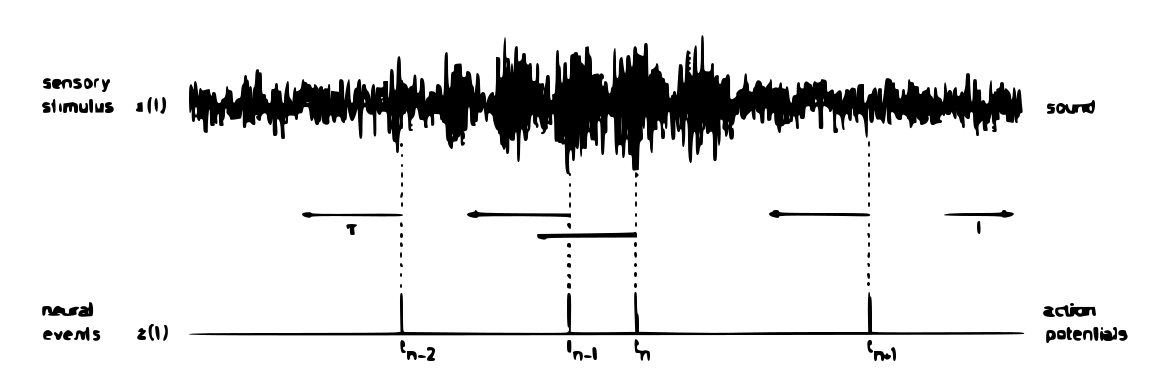
\includegraphics[scale=0.4]{pese}
	\caption{A trace of the neural activity is shown at the bottom of the image, with the action potentials marked by vertical dotted lines. On top of the image, the stimulus appears as a waveform. The lag $\tau$ is illustrated by arrows going back in time, showcasing the causal effect of the stimulus on neural activity. Adapted from \textcite{aertsenSpectrotemporalReceptiveFields1980a}.}
\end{figure}

\textcite{aertsenSpectrotemporalReceptiveFields1980} describe the PESE by means of a so-called \emph{AFT-cube}, a three-dimensional plot containing the amplitude, frequency and lag parameters of each PESE sample. Therefore, in this parametric space, each individual PESE segment is represented as a curve along the $\tau$-axis, where both the amplitude $a$ and the frequency $f$ change as the stimulus advances in the time dimension.

\subsection{STRF estimation methods}

\subsubsection{Ridge regression}
According to \textcite{theunissenEstimatingSpatiotemporalReceptive2001}, an estimation of the impulse response $h(t, x)$ in equation \eqref{impulse response} can be obtained by minimizing the expectation value of the square difference between $r$ and $\hat{r}$.
Ridge regression tries to minimize the following objective function $J$:
\begin{equation*}
	J = \min_w \norm{\mnot{k^T}\mnot{s} - r}_2^2 + \alpha \norm{\mnot{k^T}}_2^2
\end{equation*}
\noindent where $\norm{}_2$ represents the Euclidean norm and $\alpha \geq 0$ controls the amount of shrinkage

\emph{Shrinkage} is meant to prevent some weights in $k$ from becoming infinitely large or small in order to minimize the objective functions. Therefore, a penalty is applied through the term $\alpha \norm{\mnot{k^T}}_2^2$, which increases as the weights become increasingly extreme. Since $\mnot{s}$, $r$, and $\alpha$ have known values, the result of the ridge regression process is an optimal filter $\mnot{k}$ which relates the stimulus and the response.

\subsubsection{Reverse correlation}
When the stimulus is Gaussian white noise (GWN), \emph{spectrotemporal reverse correlation} can be used to estimate the STRF \parencite{kleinRobustSpectrotemporalReverse2000}. A representation of the dynamic spectrum of the stimulus portion preceding the neuron's action potential is averaged in order to obtain the STRF. The estimate becomes closer as the number of recorded action potentials increases. This process is illustrated in Figure \ref{fig:rev_corr}.

\begin{figure}
	\centering
	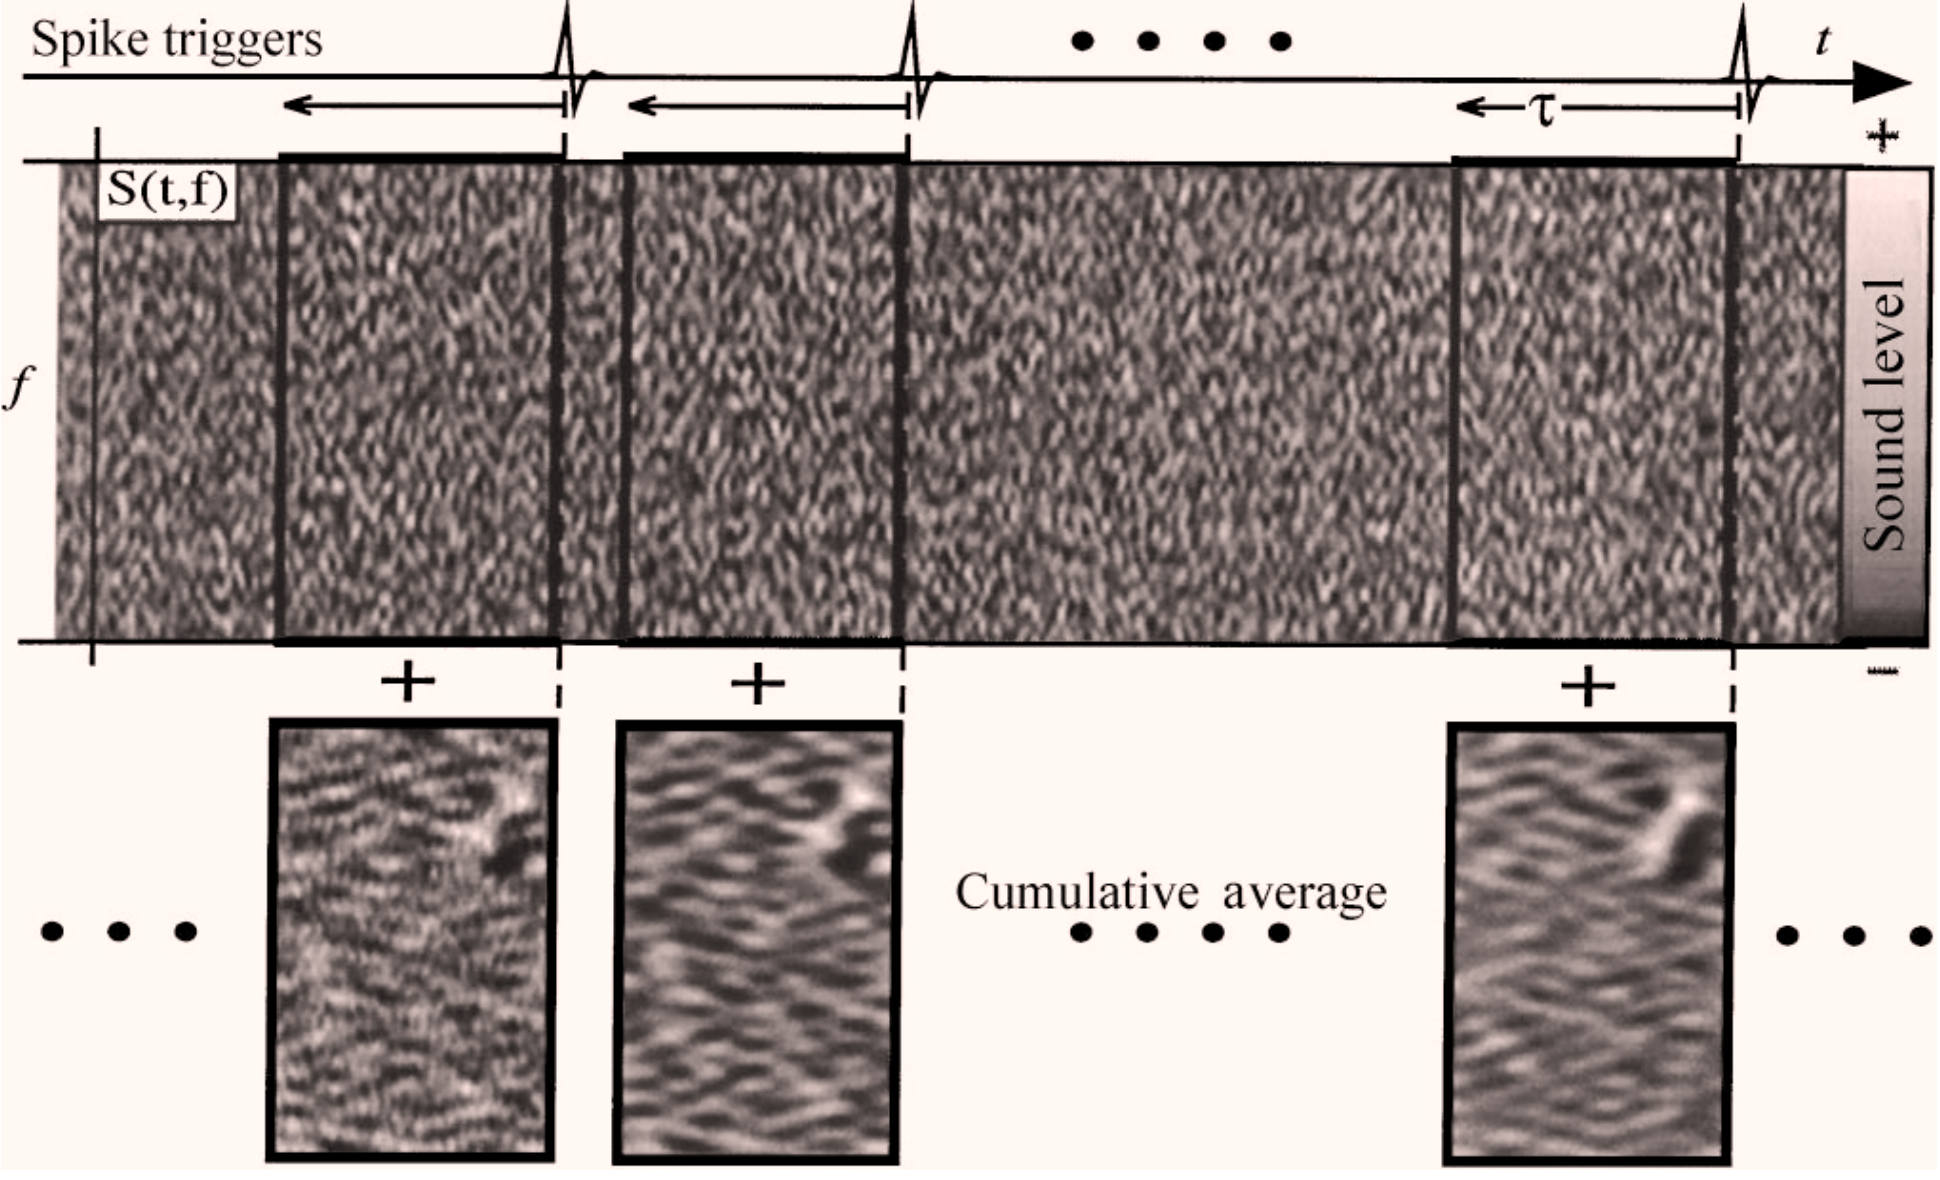
\includegraphics[scale=0.2]{reverse_corr}
	\caption{The neuronal activity is shown as the very top of the figure. Immediately below, the synchronous GWN stimulus is illustrated, along with the windows preceding the action potentials. By averaging these windows, an estimate of the STRF can be obtained. Reproduced from \textcite{kleinRobustSpectrotemporalReverse2000}.}
	\label{fig:rev_corr}
\end{figure}

